\documentclass[a4paper,10pt]{article}

\usepackage[utf8]{inputenc}
\usepackage[T1]{fontenc}
\usepackage[german]{babel}
\usepackage{amsmath}
\usepackage{multicol}
\usepackage{graphicx}
\usepackage{caption}
\usepackage{float}
\usepackage[nodayofweek,level]{datetime}
\usepackage[margin=1in,headheight=13.6pt]{geometry}

\newenvironment{Figure}
{\par\medskip\noindent\minipage{\linewidth}}
{\endminipage\par\medskip}

\usepackage{fancyhdr}
\pagestyle{fancy}
\fancyhf{}
\lhead{}
\rhead{Berner Fachhochschule}
\cfoot{\thepage}

\title{Interpolation handgeschriebener Ziffern}
\author{Bernard Jaquet}
\date{\formatdate{12}{11}{2018}}

\begin{document}
	\maketitle
	\begin{multicols}{2}
		\begin{abstract}
			
		\end{abstract}
		\section{Einleitung}
		Betrachtet man die Funktionsweise von Künstlichen Neuronalen Netzen, erkennt man eine einfache Serie von Matrixmultiplikationen und Vektoradditionen, welches einen Punkt im Problemraum in einen Punkt im Zielraum überführt. Dies ist in der Abbildung \ref{fig:feedforward} zu sehen. Im Gegensatz dazu ist zu verstehen, wie das Neuronale Netz diese Transformation macht, alles andere als trivial. Weshalb stehet in der ersten Gewichtsmatrix in der zweiten Zeile und fünften Spalte genau dieser Wert. Ist dieser Wert korrekt?
		\begin{Figure}
			\centering
			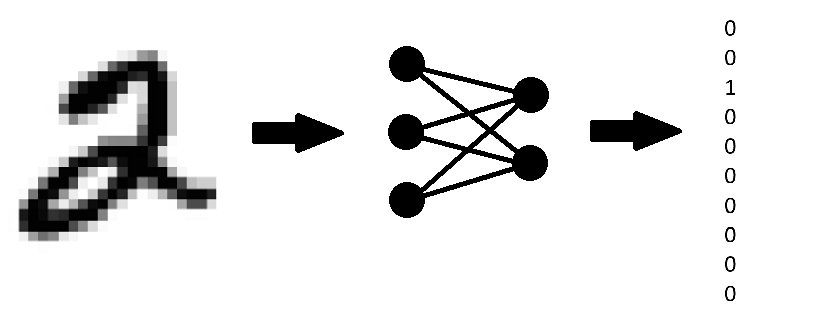
\includegraphics[width=\linewidth]{img/scribble_forward_feed.png}
			\captionof{figure}{Standard Prozess eines Neuronalen Netzes}
			\label{fig:feedforward}
		\end{Figure}
		Diese Arbeit befasst sich mit dieser Problematik und versucht gewisse ``Gedankengänge'' eines Künstlichen Neuronalen Netzes zu visualisieren. Analysiert werden die Vorgänge in einem Deep Feed-Forward Neuronal Network, welches zur Erkennung von handgeschriebenen Ziffern aus dem MNIST Datensatz trainiert wurde. Für die Visualisierung wird das Inverse des Neuronalen Netzes berechnet und gezielt mit Daten gespiesen um Bilder zu produzieren, wie sich in der Abbildung \ref{fig:feedbackwards} erkennen lässt.
		\begin{Figure}
			\centering
			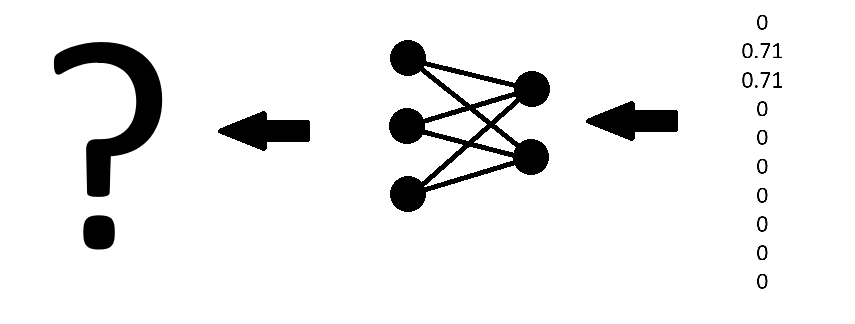
\includegraphics[width=\linewidth]{img/scribble_reverse_feed.png}
			\captionof{figure}{Intertierung des Neuronalen Neztes}
			\label{fig:feedbackwards}
		\end{Figure}
		Die Ausgabe des trainierten Neuronalen Netzes ist ein Vektor der Länge zehn, bei welchem jeder Wert der im Vektor die vom Neuronalen Netz geschätzte Wahrscheinlichkeit für das Auffinden dieser Ziffer im Ursprungsbild ist. Der Index mit dem höchsten Wert gilt als Resultat. Für das Zurückrechnen sollen in dieser Arbeit Vektoren für ``perfekte'' Ziffern, will heissen eine Eins für die entsprechende Ziffer im Vektor und Nullen für den Rest, und Vektoren für eine Mischung von Ziffern verwendet werden. Diese Interpolation der Ziffern sollen durch eine Rotation zwischen den beiden idealen Ziffern gemacht, wobei der Winkel der Rotation als Parameter für das Verhältnis der beiden Ziffern betrachtet werden kann.
		\par
		Somit ist die Fragestellung dieser Arbeit: Lassen sich die ursprünglichen Ziffern der Interpolation nach der Rückrechnung in den Problemraum erkennen?
		
		\section{Material und Methoden}
		
		\section{Ergebnisse}
		
		\section{Diskussion}
		
		\section{Literatur}
	\end{multicols}
	\newpage
	\appendix
	\section{Anhang: Resultate}
	
	\newpage
	\section{Anhang: Code}

\end{document}